% Algorithm

\section*{Introduction}

We implemented and analysed two additional algorithms in addition to the brute force algorithm that was required. One of them is the \emph{Knuth-Morris-Pratt} (KMP) algorithm with the other algorithm being \emph{Two-way String Matching}. All of the implementation was done in Python.

\section*{Brute Force Algorithm}

\subsection*{Concept}
The Brute Force Algorithm works by comparing every character in the text (haystack) and the search pattern (needle). If every character in the needle is compared successfully, then the pattern has been found successfully. If a mismatch occurs at a particular index ( Figure \ref{fig:bf_1}), then the needle is shifted up by one index, and each character is compared again ( Figure \ref{fig:bf_2}). 

\begin{figure}[H]
  \centering
  \begin{minipage}[b]{0.4\textwidth}
    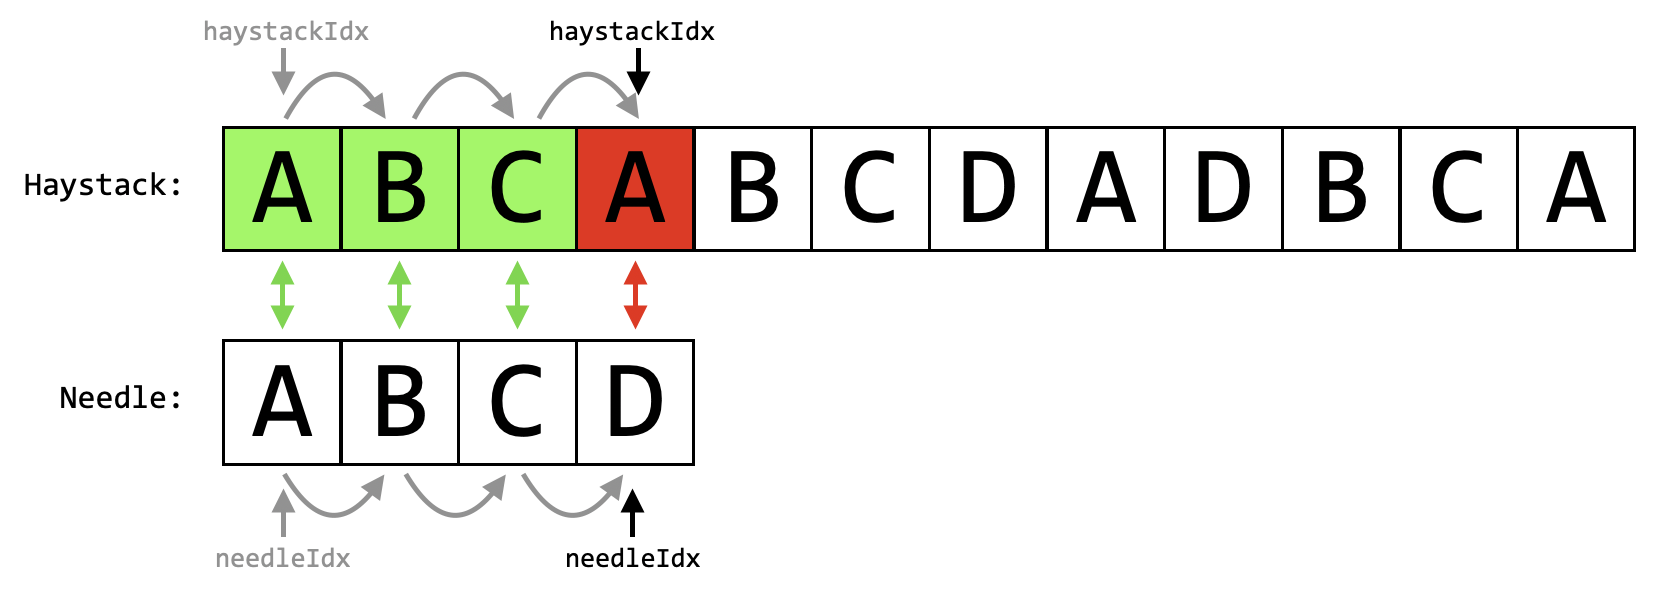
\includegraphics[width=\textwidth]{images/brute_force_1.png}
    \caption{Brute force comparisons up to first mismatch.}
    \label{fig:bf_1}
  \end{minipage}
  \hfill
  \begin{minipage}[b]{0.4\textwidth}
    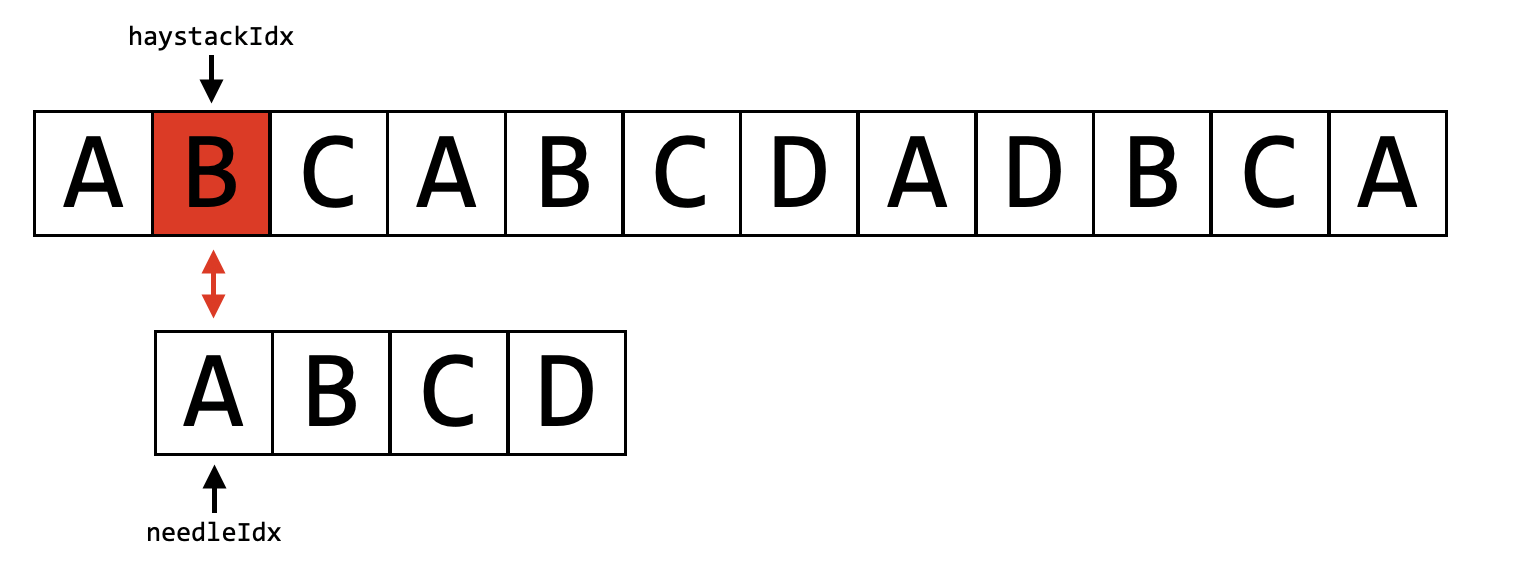
\includegraphics[width=\textwidth]{images/brute_force_2.png}
    \caption{Brute force comparison after first mismatch.}
    \label{fig:bf_2}
  \end{minipage}
\end{figure}


\subsection*{Python Implementation}

\begin{figure}[h!]
    \centering
    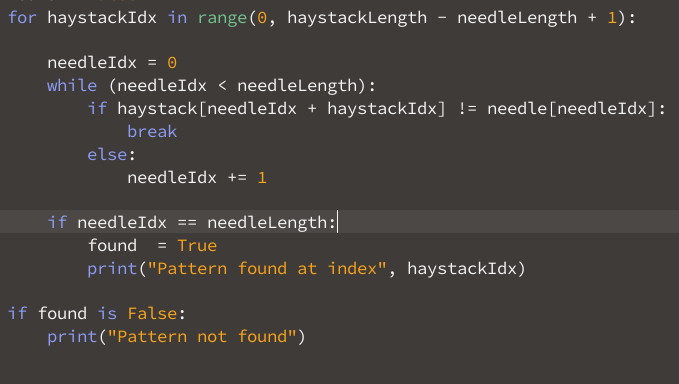
\includegraphics[width=0.50\textwidth]{images/brute_force.png}
    \caption{Code snippet of our brute force implementation}
    \label{fig:bf_code}
\end{figure}

We first initialised a \mintinline{Python}{haystackIdx} for the substring of the haystack that we are going to compare our needle with. This algorithm will begin by comparing the first letter of the text with each letter of the substring, if they are the same, it will move on to the second letter and so on until the entire needle is traversed successfully. in which case, it is matched or the letters are no longer the same, which results in the \emph{if} case and hence, breaking. Then, the position of the substring will move by one character.

Let $h, n$ be the length of the haystack and the needle respectively. For a complete search, we would need to go through all characters of the haystack. This means that we need to check $h - n + 1$ substrings. In the inner loop, we would need to compare each character of the needle to each character of the substring of the haystack. In the best case scenario, in the inner loop, the first character is never the same as the first character of the substring, i.e. the character doesn't exist in the haystack. This would just be $\mathcal{O}(1)$ in the inner loop. However, in the worst case, it would have to traverse through the entire length of the needle making the time complexity $\mathcal{O}(n)$. Hence, this means that for this brute force algorithm, the best case time complexity is $\mathcal{O}(h - n + 1)$ while the worst case is $\mathcal{O}(h - n + 1)(n)$. This worst case scenario can be simplified to being $\mathcal{O}(hn)$ and the best case being $\mathcal{O}(h)$. \\

\noindent
There is nothing to analyse for space complexity since we do not need to store any data.

\section*{Knuth-Morris-Pratt (KMP) Algorithm}

\subsection*{Concept}
One of the major drawbacks of the Brute Force Algorithm is that when a mismatch occurs, there is no built in check that prevents the algorithm from double checking characters that have previously been compared. The KMP Algorithm circumvents this inefficiency by comparing the first character of the pattern with the next occurrence of that character in the haystack. Figures \ref{fig:kmp_1} and \ref{fig:kmp_2} show an example of how KMP handles a mismatch case by skipping over previously compared characters to the next occurrence of the character `A'.

\begin{figure}[H]
  \centering
  \begin{minipage}[b]{0.4\textwidth}
    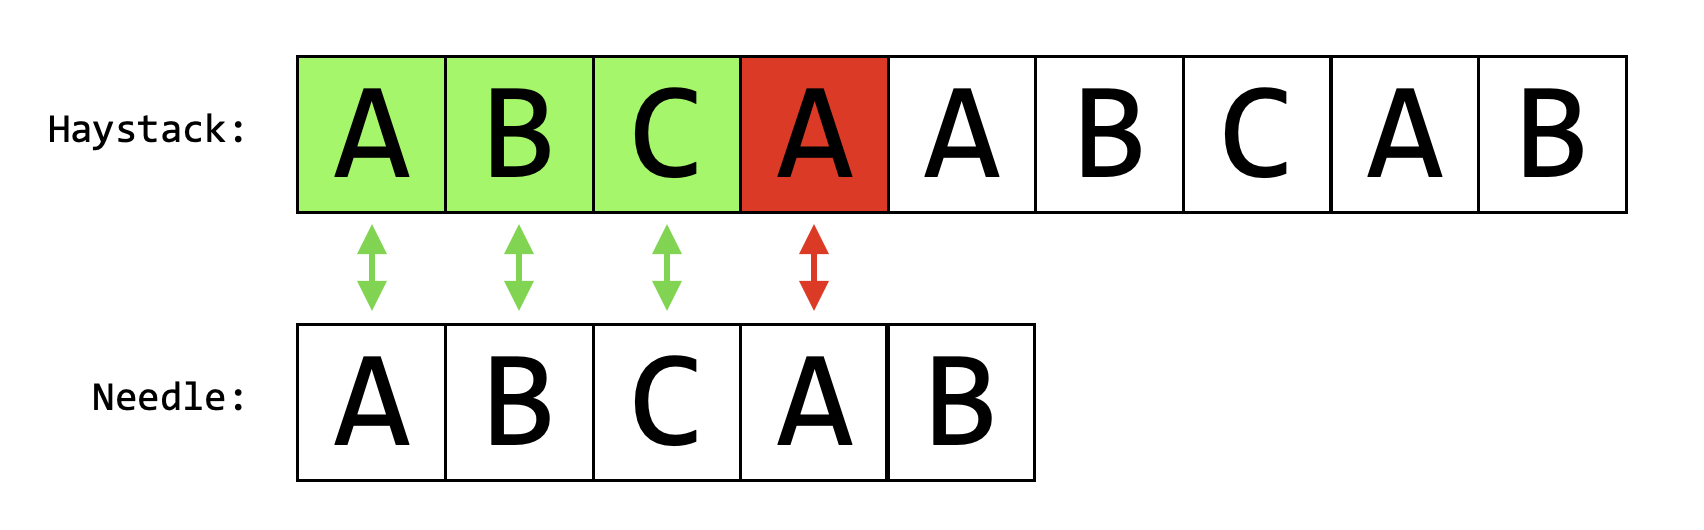
\includegraphics[width=\textwidth]{images/kmp_1.png}
    \caption{Brute force comparisons up to first mismatch.}
    \label{fig:kmp_1}
  \end{minipage}
  \hfill
  \begin{minipage}[b]{0.4\textwidth}
    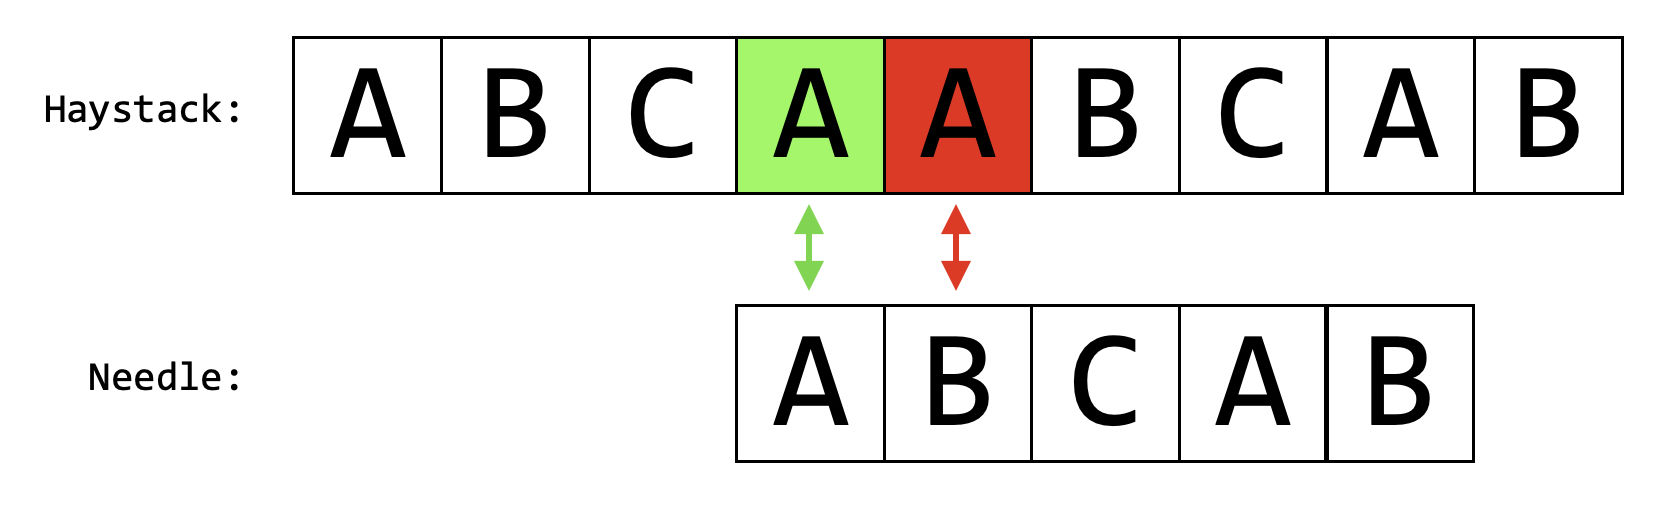
\includegraphics[width=\textwidth]{images/kmp_2.png}
    \caption{Brute force comparison after first mismatch.}
    \label{fig:kmp_2}
  \end{minipage}
\end{figure}

In order to facilitate this, the substring first needs to be preprocessed, to identify recurring patterns within the needle (referred to as prefixes and suffixes). This allows the algorithm to form a table of values that indicate the next index in the haystack that the needle should be compared to. Table \ref{tab:kmp_table} is the corresponding mismatch table for the example search pattern in Figures \ref{fig:kmp_1} and \ref{fig:kmp_2}. It indicates that if a mismatch occurs at a `B' within the haystack, we are to remain at that index, and compare it with index 1 of the needle. If a mismatch occurs at any other character, we are to remain at that index within the haystack, and compare it with index 0 of the needle. %Add figure number and reference

\begin{table}[H]
    \centering
    \begin{tabular}{|l|l|l|l|l|}
    \hline
    A & B & C & A & B \\ \hline
    0 & 0 & 0 & 0 & 1 \\ \hline
    \end{tabular}
    \caption{KMP Mismatch table.}
    \label{tab:kmp_table}
\end{table}

\subsection*{Python Implementation}

\begin{figure}[h]
    \centering
    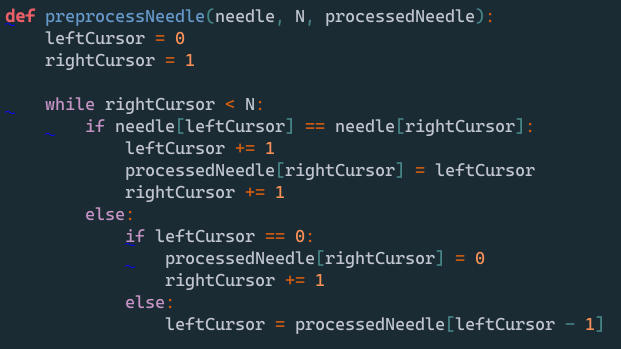
\includegraphics[width=0.50\textwidth]{images/preprocessKMP.png}
    \caption{Preprocess Function for KMP}
    \label{fig:KMP_preprocessing}
\end{figure}

The function shown in Figure \ref{fig:KMP_preprocessing} has \mintinline{Python}{processedNeedle}, an array which stores the length of the longest prefix, suffix pairs. We calculate the value such that if the \mintinline{Python}{needle[leftCursor]} and \mintinline{Python}{needle[rightCursor]} matches, we increment \mintinline{Python}{leftCursor} and assigns this value to the \mintinline{Python}{processedNeedle}. If there wasn't a match and the \mintinline{Python}{leftCursor} is pointing to the first character, we reinitialise it. The point of all of this is to find characters which form both the prefix and suffix of the needle as we iterate through the needle.

\begin{figure}[h!]
    \centering
    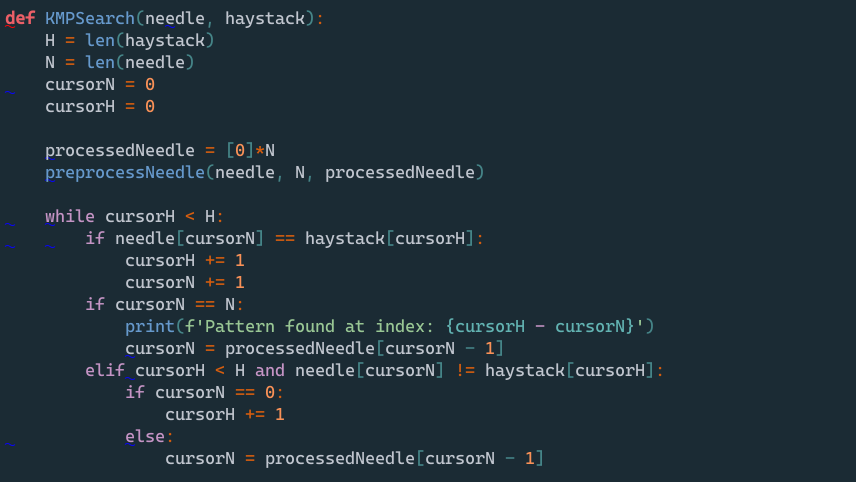
\includegraphics[width=0.50\textwidth]{images/KMP.png}
    \caption{KMP Search Function}
\end{figure}

After initialising the variables, we would need to preprocess the needle using the function in Fig 2. Since the length of the haystack and needle are $h, n$ respectively, we would begin comparison of the needle and the haystack and increment the value of the cursor while they keep matching. The \emph{if cursorN == N} indicates that all characters match with each other and the pattern is found. The benefit of KMP comes when there is a mismatch. If the mismatch happens at index $a$, this means that the first $a - 1$ characters of the needle matches with the first $a - 1$ characters of the haystack. From the preprocessing, we know that \emph{processedNeedle[a - 1]} is the number of characters that are both the prefix and suffix of that substring of the needle of length a. This means that we do not need to match the $a - 1$ characters because we know that these characters will match.

Since we do not need to do the comparison for those that are already matched, we only need to do one comparison for each character in the haystack. This means that the time complexity of the matching will be $\mathcal{O}(h)$. However, time is taken to do the preprocessing. Since we need to calculate the value of the prefix suffix pairs for each character in the needle, this would mean that the time complexity is $\mathcal{O}(n)$. Since the preprocessing and the matching happens linearly, we can say that the time complexity of the algorithm is $\mathcal{O}(h+n)$. In the problem that we are given, the best case and worst case time complexity for KMP would remain the same. This is because we want to find all occurences of the needle in the haystack. Hence, we would need to go through all the characters of the string even if a match is found in the first index. This means that the best case and worst case time complexity remains $\mathcal{O}(h+n)$.

The improvement to a linear time complexity in the worst case from $\mathcal{O}(hn)$ to $\mathcal{O}(h + n)$ comes with a tradeoff in space complexity. In the case of brute force, there is no need to store any data. However, the efficiency in KMP comes from the existence of the lookup table which is the array which tells us how many characters we do not need to match. The size of this array is equivalent to the length of the needle that we are searching for. Thus, the space complexity for KMP would be $\mathcal{O}(n)$.

\section*{Analysis}
\subsection*{Empirical Analysis}

\begin{figure}[h!]
    \centering
    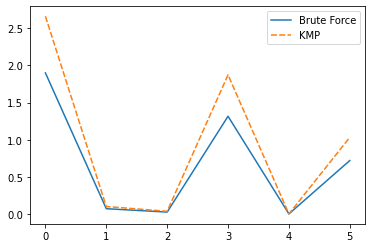
\includegraphics[width=0.50\textwidth]{images/swaggy_graph.png}
    \caption{Graph showing differences in timings}
\end{figure}

Based on the empirical analysis that we have done above, we can see that for most cases that we tested. Brute force actually take a shorter amount of time compared to KMP even though we have mentioned above that KMP should theoretically be faster since it's time complexity is $\mathcal{O}(h+n)$ in comparison to the worst case time complexity of Brute Force which is $\mathcal{O}(hn)$. However, this worst case scenario would occur only when the comparison for the substring is the same until the last character. For example, a needle of "AAAC" and a haystack filled completely with "A"s. However, this is not the case that we're dealing with in this problem and neither is this something that will reasonably happen in a real search. On average, the number of comparisons that would have to be done everytime the character shifts is much less than $n$. This is why it is faster than KMP in the experiment that we have done since the KMP algorithm would still have a time complexity of $\mathcal{O}(n+m)$ even in the best case.

\begin{figure}[h!]
    \centering
    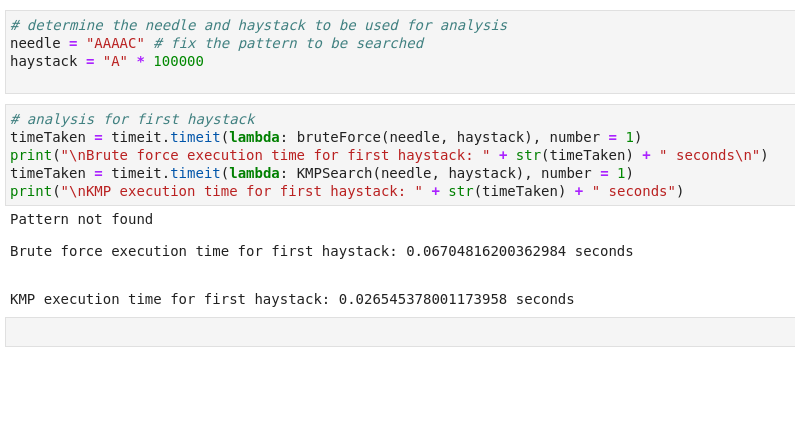
\includegraphics[width=0.50\textwidth]{images/worst_case.png}
    \caption{Timings}
\end{figure}

As has been mentioned, in this case, it is certainly faster for KMP than Brute Force to run. However, this is unrealistic since it is extremely improbable to encounter this in any string search scenario for a DNA